\documentclass[]{article}

\usepackage{graphicx}
\usepackage{float}
\usepackage{indentfirst}
\usepackage{parskip}
\setlength\parindent{24pt}
%opening
\title{Particle filter -- report}
\author{Dhasharath Shrivathsa \& Katie Butler}

\begin{document}
\maketitle

\begin{abstract}
Particle filters are a useful way to describe a set of discrete hypotheses $\{\beta_0, \beta_1 ...\beta_n\}$ to approximate $(\alpha')$ some truth about the world $\alpha$. This process occurs by iteratively updating each $\beta$ with data $D$ as it comes in. The Bayesian approach is applicable here, as we can frame each $D$ as a Bayesian update on the set of $\beta$'s, $P(\beta|D)$
\end{abstract}
\begin{figure}[H]
	\centering
	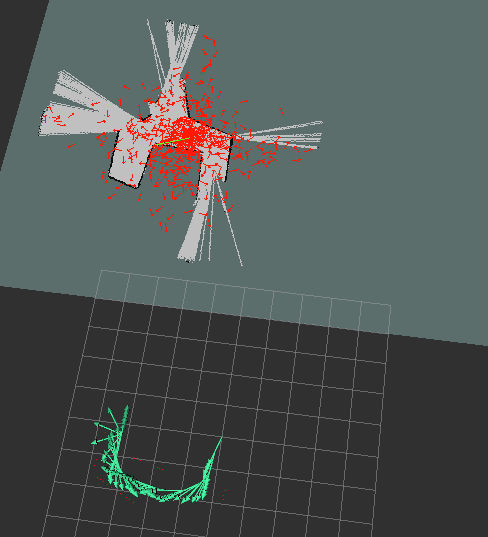
\includegraphics[width=0.7\linewidth]{pf_convergence}
	\caption{Particle filter localization demo}
	\label{fig:pfconvergence}
\end{figure}

\section{Goal}
The goal for this project was to have a working basic particle filter with as few assumptions made about the problem as possible. I decided to go for a 2-day from-the-ground rewrite of a particle filter to identify inefficiencies and work out how one really works, including the hairy coordinate frame stuff that Paul somewhat boxed away.

This was a success
\section{Problem solving description}
We can decompose the particle filter into several simple steps:
\subsection{Initialization}
\paragraph{Initialize map $M$}
The map is recieved from the ROS service \verb|map_server|, and is wrapped in an \verb|OccupancyField| so we can have python bindings to be able to query the map nicely. 

This is worth noting because my implementation differs from Paul's greatly (see \verb|scripts/my_pf.py|). One important distinction is how the single method that \verb|OccupancyField| implements, \verb|get_distance_to_closest_obstacle|, has a different time complexity. Paul's implementation uses a $O(1)$ time, as he wraps it in a \verb|NearestNeighbors(n_neighbors=1)| classifier. My implementation is $O(n)$ because I didn't need the speed. It can be converted to $O(1)$ trivially.
\paragraph{Initialize particles $\{\beta\}$}
To spread out the initial set of hypotheses, we sample uniformly across the convex hull of the points in the occupancy field. The convex hull is computed with the initialization of the \verb|OccupancyField| class, and we build a bounding box and sample across that, taking only what lies within the hull up to \verb|n_particles|. This gives us $\{\beta\}$ with equal confidence weights
\subsection{Callbacks}
\paragraph{Odometry}
As the robot moves, we'd like to update all our hypotheses. The callback \verb|update_particles_with_odom| handles relative distance and angle transforms every time the robot moves greater than some amount. This math requires a small amount of angle thinking, as moving in the $x$-direction when $\theta = 0$ is not the same as when $\theta = 90$.
\paragraph{Laser scans $L$}
As the robot recieves new laser scans, we project each scan onto each $\beta$, measuring its error, and performing a confidence update on each. In the existing model, we square the error and divide each $\beta$ (higher weights are better particles). 

This lets us encode the whole set of sensor readings into each $\beta$, as $P(\beta, L_{t-1}...)$ is the weight of $\beta$

\subsection{Utility and ROS interface}
\paragraph{Visualization} Each $\beta$ is a \verb|Pose| in a \verb|PoseArray|. \verb|alpha_pose/alpha_prime|, our best guess, is a pose from $\{\beta\}$, the one with the most weight. I do not calculate the origin-map-frame-to-odom-frame transform, as that's a debugging detail in the problem description
\section{Design decisions}
To maintain a rugged filter and to enable post-localization unceartainty, the code only samples across a fat-tailed cauchy distribution.

It considers all Laser scans

It considers points only valid if they're within the convex hull of the occupied points on the map
\section{Challenges}
The timeframe was the main challenge, as I did the project twice over, first with a partner, and then as a time-constrained implementation exercise. Of the two, the time-constrained one was much harder and I learned more technical and implementation details from that. The partner-based project was also interesting, as I was forced to refine my definitions, at the end taking up no more than a single side of a4 written in sharpie.
\section{Improvements}
I'd want to find ways to enforce multi-modality and parameterize more things to find out how to tune the filter.

Improvements from more sensors would be nice.

I really want to create a cohesive ROS class structure that makes it easier to write and debug code (see \verb|warmup_project/scripts/classes.py|). I would like to rewrite this in C as python/rospy flaws became apparent.
\end{document}
